% !TEX TS-program = XeLaTeX
% use the following command:
% all document files must be coded in UTF-8
\documentclass[spanish]{textolivre}
% build HTML with: make4ht -e build.lua -c textolivre.cfg -x -u article "fn-in,svg,pic-align"
\usepackage{caption}   % Para legendas
\usepackage{float}
\usepackage{array}
%\usepackage{longtable}
%\usepackage{makecell}

\journalname{Texto Livre}
\thevolume{18}
%\thenumber{1} % old template
\theyear{2025}
\receiveddate{\DTMdisplaydate{2024}{12}{10}{-1}} % YYYY MM DD
\accepteddate{\DTMdisplaydate{2025}{4}{4}{-1}}
\publisheddate{\DTMdisplaydate{2025}{6}{15}{-1}}
\corrauthor{Alfons Medina Cambrón}
\articledoi{10.1590/1983-3652.2025.56425}
%\articleid{NNNN} % if the article ID is not the last 5 numbers of its DOI, provide it using \articleid{} commmand 
% list of available sesscions in the journal: articles, dossier, reports, essays, reviews, interviews, editorial
\articlesessionname{articles}
\runningauthor{Medina Cambrón y Ballano Macías} 
%\editorname{Leonardo Araújo} % old template
\sectioneditorname{Hugo Heredia Ponce}
\layouteditorname{Saula Cecília}

\title{El papel de la investigación española en la producción científica internacional sobre competencia digital docente (2010-2023): tendencias, problemáticas y retos}
\othertitle{O papel da pesquisa espanhola na produção científica internacional sobre competência digital docente (2010-2023): tendências, problemáticas e desafios}
% if there is a third language title, add here:
\othertitle{The role of Spanish research in the international scientific production on teachers’ digital competence (2010-2023): trends, problems, and challenges}

\author[1]{Alfons Medina Cambrón~\orcid{0000-0001-8886-4564}\thanks{Email: \href{mailto:alfonsomc@blanquerna.url.edu}{alfonsomc@blanquerna.url.edu}}}
\author[1]{Sonia Ballano Macías~\orcid{0000-0002-6322-1383}\thanks{Email: \href{mailto:soniabm@blanquerna.url.edu}{soniabm@blanquerna.url.edu}}}
\affil[1]{Universidad Ramon Llull, Facultad de Comunicación y Relaciones Internacionales Blanquerna, Barcelona, España.}

\addbibresource{article.bib}
% use biber instead of bibtex
% $ biber article


% if you use multirows in a table, include the multirow package
\usepackage{multirow}

% provides sidewaysfigure environment
\usepackage{rotating}

% CUSTOM EPIGRAPH - BEGIN 
%%% https://tex.stackexchange.com/questions/193178/specific-epigraph-style
\usepackage{epigraph}
\renewcommand\textflush{flushright}
\makeatletter
\newlength\epitextskip
\pretocmd{\@epitext}{\em}{}{}
\apptocmd{\@epitext}{\em}{}{}
\patchcmd{\epigraph}{\@epitext{#1}\\}{\@epitext{#1}\\[\epitextskip]}{}{}
\makeatother
\setlength\epigraphrule{0pt}
\setlength\epitextskip{0.5ex}
\setlength\epigraphwidth{.7\textwidth}
% CUSTOM EPIGRAPH - END

% to use IPA symbols in unicode add
%\usepackage{fontspec}
%\newfontfamily\ipafont{CMU Serif}
%\newcommand{\ipa}[1]{{\ipafont #1}}
% and in the text you may use the \ipa{...} command passing the symbols in unicode

% LANGUAGE - BEGIN
% ARABIC
% for languages that use special fonts, you must provide the typeface that will be used
% \setotherlanguage{arabic}
% \newfontfamily\arabicfont[Script=Arabic]{Amiri}
% \newfontfamily\arabicfontsf[Script=Arabic]{Amiri}
% \newfontfamily\arabicfonttt[Script=Arabic]{Amiri}
%
% in the article, to add arabic text use: \textlang{arabic}{ ... }
%
% RUSSIAN
% for russian text we also need to define fonts with support for Cyrillic script
% \usepackage{fontspec}
% \setotherlanguage{russian}
% \newfontfamily\cyrillicfont{Times New Roman}
% \newfontfamily\cyrillicfontsf{Times New Roman}[Script=Cyrillic]
% \newfontfamily\cyrillicfonttt{Times New Roman}[Script=Cyrillic]
%
% in the text use \begin{russian} ... \end{russian}
% LANGUAGE - END

% EMOJIS - BEGIN
% to use emoticons in your manuscript
% https://stackoverflow.com/questions/190145/how-to-insert-emoticons-in-latex/57076064
% using font Symbola, which has full support
% the font may be downloaded at:
% https://dn-works.com/ufas/
% add to preamble:
% \newfontfamily\Symbola{Symbola}
% in the text use:
% {\Symbola }
% EMOJIS - END

% LABEL REFERENCE TO DESCRIPTIVE LIST - BEGIN
% reference itens in a descriptive list using their labels instead of numbers
% insert the code below in the preambule:
%\makeatletter
%\let\orgdescriptionlabel\descriptionlabel
%\renewcommand*{\descriptionlabel}[1]{%
%  \let\orglabel\label
%  \let\label\@gobble
%  \phantomsection
%  \edef\@currentlabel{#1\unskip}%
%  \let\label\orglabel
%  \orgdescriptionlabel{#1}%
%}
%\makeatother
%
% in your document, use as illustraded here:
%\begin{description}
%  \item[first\label{itm1}] this is only an example;
%  % ...  add more items
%\end{description}
% LABEL REFERENCE TO DESCRIPTIVE LIST - END


% add line numbers for submission
%\usepackage{lineno}
%\linenumbers

\begin{document}
\maketitle

\begin{polyabstract}
\begin{abstract}
Este artículo tiene como objetivo situar la investigación española relativa a la competencia digital docente (CDD) en el contexto internacional. Se han analizado en profundidad un total de 580 publicaciones en revistas indexadas en Web of Science y Scopus durante el periodo 2010-2023. Los resultados ponen de manifiesto un crecimiento exponencial durante las últimas dos décadas en dicha temática, el protagonismo indiscutible de la investigación española (60 \% del total de publicaciones) y una elevada concentración de la difusión científica en pocas revistas académicas. Se identifica como ámbito de estudio prioritario la (auto)percepción del profesorado o futuro profesorado abordándose, casi exclusivamente, mediante encuestas con poblaciones dispersas y muestras muy reducidas y no probabilísticas. Por tanto, se hace necesario trabajar con muestras más representativas y metodologías cualitativas que permitan dar coherencia a una legislación sobre CDD que se ha centrado en la educación no universitaria, mientras que la investigación sigue tomando como objeto de estudio mayoritario al alumnado y al profesorado universitario.

\keywords{Competencia digital docente \sep Investigación educativa \sep Metodologías \sep TIC}
\end{abstract}

\begin{portuguese}
\begin{abstract}
Este artigo tem como objetivo situar a produção científica espanhola relacionada à competência digital docente (CDD) no contexto internacional. Foram analisadas em profundidade um total de 580 publicações em revistas indexadas na Web of Science e Scopus no período de 2010-2023. Os resultados revelam um crescimento exponencial nas últimas duas décadas sobre este tema, o protagonismo indiscutível da pesquisa espanhola (60\% do total de publicações) e uma elevada concentração da difusão científica em poucas revistas acadêmicas. A (auto)percepção dos professores ou futuros professores é identificada como uma área prioritária de estudo, sendo abordada quase exclusivamente através de pesquisas com populações dispersas e amostras muito reduzidas e não probabilísticas. Portanto, é necessário trabalhar com amostras mais representativas e metodologias qualitativas que permitam dar coerência à legislação sobre CDD que tem se centrado no ensino não universitário, enquanto a pesquisa continua a ter como principal objeto de estudo os estudantes e professores universitários.

\keywords{Competência digital docente \sep Pesquisa educacional \sep Metodologias \sep TIC}
\end{abstract}
\end{portuguese}

\begin{english}
\begin{abstract}
 The aim of this article is to place Spanish research on teacher digital competence within the international context. The research includes an in-depth analysis of 580 publications indexed in the Web of Science and Scopus databases from the period 2010-2023. The results show an exponential growth over the last two decades in this area, highlighting the undeniable prominence of Spanish research (accounting for 60\% of the total publications) and indicating a high concentration of scientific dissemination in a few academic journals. The (self-)perception of teachers or future teachers has been identified as a priority area of study, being addressed almost exclusively through surveys conducted with dispersed populations and very small, non-probabilistic samples. Therefore, it becomes necessary to work with more representative samples and qualitative methodologies that can provide coherence to legislation on teacher digital competence, which has focused on non-university education, while research predominantly takes students and university teachers as its main subjects of study.

\keywords{Teacher digital competence \sep Educational research \sep Methodologies \sep ICT}
\end{abstract}
\end{english}

\end{polyabstract}

\section{Introducción}\label{sec-1}
La introducción y asentamiento de las Tecnologías de la Información y la Comunicación (en adelante, TIC), ha revolucionado la manera en que concebimos los procesos comunicativos y educativos, situando la competencia digital como una dimensión clave para el aprendizaje a lo largo de la vida \cite{comisioneuropea2006}. El impacto de las TIC en la educación ya sea formal, no formal e informal, ha sido, de forma recurrente, motivo de interés para las ciencias sociales. La OCDE inició en 1997 el proyecto “Definition and Selection of Competencies” con la intención de crear un marco teórico para definir las competencias necesarias para encarar los retos de una sociedad en transformación y donde ya se vislumbraba la importancia de la tecnología  \cite{ocde2005}. De igual modo, el Parlamento Europeo y el Consejo \cite{comisioneuropea2006}, describen las competencias como la integración de actitudes, capacidades y conocimientos; señalando la competencia digital como una dimensión clave para el desarrollo personal, la inclusión social, la ocupabilidad y la ciudadanía activa. A partir de ese momento, los esfuerzos por definir las competencias clave se sitúan en un contexto marcado por el protagonismo creciente de las TIC y el desarrollo de las redes sociales; donde las nuevas desigualdades ya no se basan tanto en el acceso al entorno digital, sino en la calidad y aprovechamiento de su uso \cite{buckingham2020, medina2015}.

Más recientemente, el avance de la inteligencia artificial (en adelante, IA) vuelve a situar el foco de atención en la necesidad de garantizar la competencia digital de la población en general, pero también de docentes y alumnado en particular, bajo la certeza de que los procesos de enseñanza-aprendizaje deben contextualizarse, situarse y convivir con los algoritmos \cite{unesco2019}. La investigación y marcos de referencia generados sobre competencia y competencia digital se ha focalizado en diferentes agentes: la población adulta, el alumnado y el profesorado de diversos niveles educativos. Este artículo abordará exclusivamente la competencia digital docente (en adelante, CDD).

\subsection{Situando la noción de competencia digital docente (CDD) en España}\label{sec-1.1}
Se puede entender por CDD la integración de saberes, destrezas, habilidades y actitudes que cualquier docente debe poner en juego, de manera simultánea y ayudado de las tecnologías digitales. La noción de CDD es una de las acepciones que viene a sumarse a conceptos como alfabetización informacional, digital o mediática, competencia mediática o digital o, incluso, competencia profesional docente y que han contribuido a enriquecer, pero también a fragmentar o dispersar, la literatura científica en torno al objeto de estudio \cite{aguaded2022, area2012, gutierrez2012}.

Esta diversidad de conceptos irá también acompañada de una diversidad de enfoques: los primeros, centrados especialmente en las habilidades técnicas relacionadas con el uso de herramientas digitales; los segundos, ampliando el foco, no solo a la importancia de las competencias digitales instrumentales, sino también metodológicas \cite{barragan2021, generalitat2018}. Existen también enfoques que sitúan la competencia digital en la articulación de múltiples alfabetizaciones que tienen por objeto común la lectoescritura, así como la comprensión y uso crítico de los medios y plataformas de comunicación tecnológicas y digitales \cite{buckingham2020}.

La revisión del estado de la cuestión permite establecer, durante las dos últimas décadas y para el caso español, diferentes fases temporales que muestran la evolución de la investigación en CDD en función de las dimensiones que han resultado prioritarias en cada momento: 1) digitalización de los centros; 2) introducción de procesos de innovación pedagógica digital; 3) posesión de las competencias digitales por parte del alumnado; 4) fomento de la detección, aceptación y adquisición de la CDD entre el profesorado como premisa necesaria para conseguir lo anterior; y, en última instancia y más recientemente, 5) establecimiento de un marco propio para la certificación de la CDD. La consolidación de marcos de referencia ha reorientado de manera acelerada los enfoques centrados en la evaluación de la percepción sobre la CDD desde un punto de vista más cualitativo hacia enfoques centrados en la definición de categorías, niveles e indicadores para su acreditación \cite{caberoalmenara-palacios2020}. En este punto, es evidente que la velocidad a la que el desarrollo de las TIC sigue impactando en todas las esferas de la sociedad sumado a las incertidumbres y transformaciones urgentes en las prácticas educativas que han tenido lugar a partir de la COVID-19, hace útil y necesario un análisis de la literatura científica de máximo impacto sobre CDD que permita analizar y reorientar escenarios de futuro.

\subsection{Marcos de referencia de la CDD en España}\label{sec-1.2}
La documentación generada a nivel internacional sobre el concepto de competencia \cite{ocde2005, comisioneuropea2006} está en la base del trabajo de la UNESCO para situar las competencias TIC de los docentes \cite{unesco2008, unesco2018}. Aunque existan algunas experiencias entre 2001 y 2006 en Quebec, Australia, Dinamarca o Chile \cite{carrera2012}, la legislación y la investigación sobre CDD tendrá un gran impulso a partir de la segunda década de este siglo. En España, el desarrollo normativo sobre la CDD se ha ido configurando progresivamente a partir de un conjunto de propuestas tanto a nivel estatal como internacional \cite{caberoalmenara-palacios2020, lazaro2019} que han permitido definir su significado y alcance, sus dimensiones y el diseño de indicadores para su evaluación y acreditación. Uno de los documentos más influyentes ha sido el \textit{Marco Europeo de Competencia Digital para Docentes -- DigCompEdu} \cite{caberoalmenaraetal2020, redecker2017}.

En el caso de España, INTEF publicó en 2014 un primer documento del Marco Común de CDD, actualizado en 2017 \cite{intef2017}. A su vez, algunas Comunidades Autónomas han generado documentación para la elaboración de un marco de referencia de la CDD; por ejemplo, en el caso de Cataluña, entre otros aspectos, en la identificación de variables e indicadores de las competencias digitales \cite{generalitat2018}. Estos trabajos previos nos ofrecen, para el caso español, en 2020, un primer resultado sobre el marco de referencia de la CDD para la docencia no universitaria, actualizado nuevamente en 2022 \cite{boe2020, boe2022a}. El documento marco actual se ha configurado a partir de propuestas regionales, estatales y europeas sobre competencia digital; entre ellas la hoja de ruta propuesta por la Comisión Europea para el periodo 2021-2027, que requiere disponer de profesorado competente en el uso de las TIC \cite{comisioneuropea2020}. Finalmente, también se dispone, desde 2022, de un documento común sobre la certificación, acreditación y reconocimiento de la CDD \cite{boe2022b}. Por tanto, tanto los marcos de referencia como la rúbrica para su evaluación tienen como público objetivo el profesorado no universitario.


\subsection{Tendencias de la investigación sobre CDD; Retos y problemáticas}\label{sec-1.3}
Los primeros enfoques sobre la CDD dejaban constancia de que la simple introducción de tecnología en los centros educativos no conllevaría la adquisición de competencias por parte del alumnado. La prioridad y las energías se centraban en la dotación tecnológica de los centros y la obtención de las competencias necesarias para que los estudiantes se desenvolviesen en una sociedad digital \cite{carrera2012, mork2014}. La adquisición de la CDD era prácticamente una consecuencia sobrevenida de lo anterior y, más allá del diseño curricular, la adopción de las TIC en las aulas era, en muchos casos, una cuestión de voluntarismo \cite{medina2015}.

Por otra parte, aunque el problema de la dotación tecnología de los centros educativos ya se había apuntado \cite{busquet2018}, será la situación vivida con el COVID-19 la que lo volverá a poner de manifiesto, añadiéndose, además, las dificultades de acceso a las TIC de grupos socialmente desfavorecidos \cite{hernandezortega2021}. También surgen investigaciones que reclaman un giro significativo hacia el profesorado, entendiendo la competencia digital como competencia pedagógica digital \cite{alvarez2015, area2012, lazaro2019}. Gran parte de la investigación sobre CDD conecta con el desarrollo progresivo de marcos de referencia para identificar, evaluar y, más recientemente, acreditar la CDD \cite{castaneda2018, colasbravo2021, martinezbravo2021}.

Una de las aproximaciones de investigación más recurrentes en los últimos años ha sido determinar la percepción de la competencia digital del profesorado o futuro profesorado \cite{alvarez2015, barragan2021, carrera2012, domingocoscollola2020, ramirez2012}. En este sentido, el uso de las TIC y la CDD han sido prácticamente considerados como sinónimos, tanto en la investigación como en la documentación generada por las administraciones \cite{carrera2012, generalitat2018}, aunque ya se había apuntado que el uso no determina la competencia ni la competencia comporta necesariamente el uso en el aula \cite{ramirez2012}. En los últimos años, las revisiones sistemáticas sobre CDD apuntan hacia una investigación centrada en estudios cuantitativos que parten de instrumentos de autopercepción de la competencia digital focalizados en la educación superior \cite{barragan2021, colasbravo2021, fernandezbatanero2021, zhao2021, peters2022}. La presente investigación revisa y analiza la producción científica española sobre CDD, identificando los métodos de investigación que la sustentan y señalando tendencias, desafíos y elementos de discusión para futuras líneas de investigación y de reflexión sobre la CDD.

\subsection{Objetivos e hipótesis}\label{sec-1.4}
El objetivo principal de este artículo es situar la investigación española en materia de CDD en el contexto internacional. Como objetivo específico se pretende identificar la metodología y las técnicas de investigación más utilizadas en esta área de conocimiento. Se observará, también, si existen cambios de tendencia en la investigación sobre CDD en el periodo de pandemia y postpandemia. Se parte de las siguientes hipótesis:

\begin{itemize}
    \item H1 -- La investigación española tiene un impacto significativo en la producción científica internacional sobre CDD.
    \item H2 -- Para evaluar la CDD se usan, mayoritariamente, encuestas no probabilísticas, poco significativas y con muestras excesivamente dispersas.
    \item H3 -- El periodo de pandemia y postpandemia conlleva un crecimiento significativo de la producción científica sobre CDD.
\end{itemize}

\section{Metodología}\label{sec-2}
En primer lugar, se han revisado los principales documentos legislativos y académicos en el contexto nacional e internacional para sustentar teóricamente el concepto y la evolución de la CDD. A continuación, se ha realizado una revisión de la literatura científica relativa a la CDD, teniendo en cuenta y adaptando la metodología propuesta por PRISMA \cite{aguaded2022, fuentecobo2018, georgereyes2021, peters2022}. Las dos fuentes que se han utilizado para la recopilación y análisis de la producción científica han sido Web of Science y Scopus; aplicando, en todos los casos, estrategias propias de la búsqueda parametrizada para la correcta aplicación y gestión de los criterios de inclusión y exclusión adoptados, con un periodo temporal 2010-2023. Dicho periodo, se explica por: a) la influencia de normativas internacionales al respecto, b) la legislación que se ha generado en el caso español durante esta década, c) el auge considerable de la digitalización e impulso de las TIC durante el periodo y d) para calibrar el efecto de la pandemia en la última parte del periodo. Se ha establecido como parámetro la recuperación de artículos en castellano e inglés publicados en acceso abierto.  

Para llevar a cabo la recopilación documental se ha utilizado la ecuación de búsqueda \textit{“Digital competence and teach*”}, que incorpora el concepto relativo a competencia digital o digital competence y añade el operador de truncamiento a la raíz \textit{“teach” (teach*)} para poder recuperar un mayor número de resultados. Las búsquedas en Web of Science parten de la presencia de dichos conceptos en el resumen, teniendo como referencia los artículos que aparecen en \textit{Science Citacion Index Expanded, Social Sciences Citation Index} y \textit{Arts and Humanities Citation Index}; mientras que, en el caso de Scopus, el criterio de búsqueda se centra en el título, palabras clave y resumen.

Si bien es cierto que existen conceptos similares que pueden considerarse alternativos a la noción de competencia digital (competencia mediática, alfabetización digital, formación TIC, entre otros), existe un cierto consenso en el uso mayoritario de la noción de competencia digital, tal y como se ha señalado en apartados anteriores. Pese a ello, se optó por la realización de una búsqueda previa de control en las revistas españolas presentes en Q1 y Q2 de Scopus en el ámbito de Comunicación y Educación, para comprobar que, efectivamente, la práctica totalidad de los artículos recuperados con otros conceptos quedaban también recuperados en la ecuación de búsqueda propuesta. Seguidamente, se exponen los criterios de inclusión/exclusión que se llevaron a cabo en una primera fase (\Cref{tab-1}).

%--- CÓDIGO TABELA 1 ---%
\begin{table}[h!]
\centering
\caption{Criterios de inclusión/exclusión.}
\begin{tabular}{@{}lp{10.75cm}@{}}
\toprule
Tipología de documento & Inclusión: Artículos de revista científica \newline Exclusión: Monografías \\ 
Fuente de investigación & Inclusión: Scopus Q1 y Q2 (Educación/Comunicación) y Web of Science \newline Exclusión: artículos duplicados \\ 
Idioma & Castellano e inglés \\ 
Periodo & 2010--2023 \\ 
Ecuación de búsqueda & Para Scopus se ha utilizado la ecuación de búsqueda: \textit{``digital competence and teach*''} en título, resumen y palabras clave. Para Web of Science, se ha utilizado también la misma ecuación en el resumen \\ 
Estado del documento & Acceso abierto \\
\bottomrule
\end{tabular}
\source{Elaboración propia.}
\label{tab-1}
\end{table}

En la siguiente fase se pasó a analizar en profundidad el contenido de los artículos, en concreto a partir del resumen, el apartado metodológico y las conclusiones. En este análisis se descartaron los artículos sobre competencia digital del alumnado o de otros colectivos (familias o ciudadanía en general). Los criterios de inclusión aplicados en la lectura y análisis de los artículos seleccionados fueron:

\begin{itemize}
\item Artículos sobre CDD basados en la percepción propia del profesorado o bien en la percepción o evaluación llevada a cabo por otros agentes: estudiantes, investigadores u otros.
\item  Artículos sobre CDD fundamentados en la evaluación o percepción del alumnado que cursa estudios universitarios habilitadores para ejercer como docentes: en el artículo han sido denominados como futuro profesorado.
\item  Investigaciones teóricas o aplicadas sobre CDD que presentan revisiones sistemáticas sobre la temática analizada, evaluaciones de instrumentos o bien propuestas de conceptualización de la CDD.
\end{itemize}

La primera selección recuperada comprendía un total de 1453 artículos, 449 en Web of Science (WoS) y 1004 en Scopus (ver \Cref{fig-1}). Esta fue revisada para eliminar los resultados que no se correspondían con los criterios de búsqueda aplicando los procedimientos descritos. Finalmente, se obtuvo una muestra de 580 artículos para su análisis en profundidad. 

\begin{figure}[h!]
    \begin{minipage}{.9\textwidth}
    \centering
    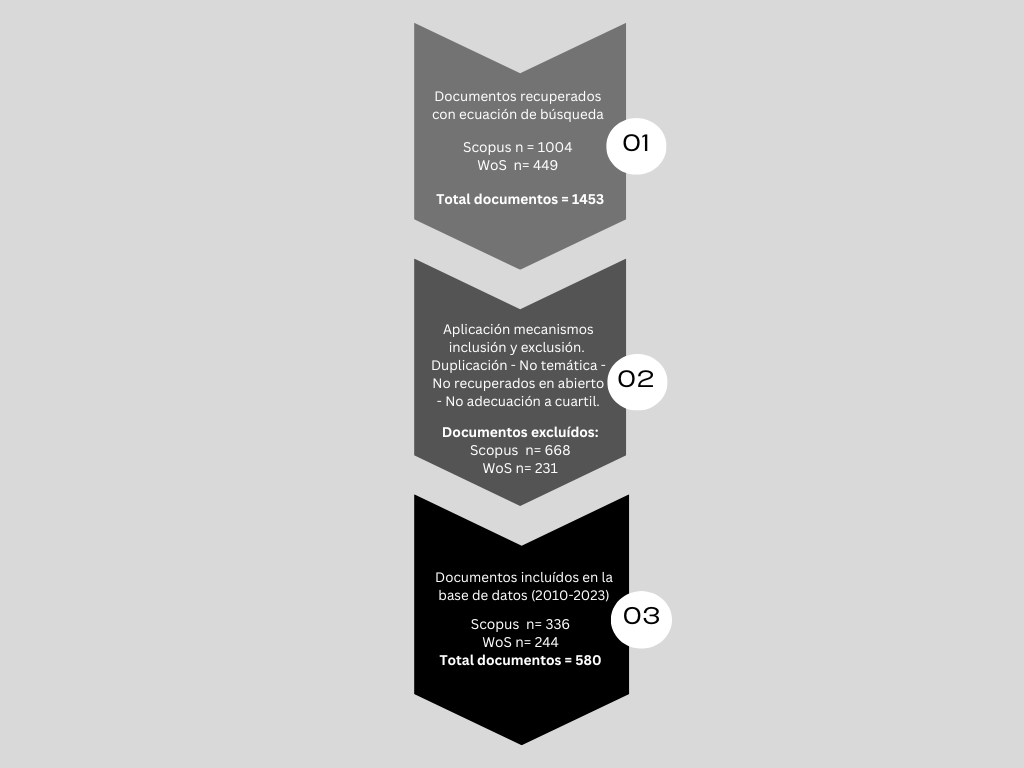
\includegraphics[width=\linewidth]{images/image1.png}
    \caption{Diagrama de flujo. Criterios de inclusión/exclusión.}
    \label{fig-1}
    \source{Elaboración propia.}
    \end{minipage}
\end{figure}

El análisis de contenido de los 580 artículos ha permitido la elaboración de una base de datos partiendo de 18 variables de análisis (\Cref{tab-2}). Algunas variables no han presentado problemas de clasificación como la denominación de la revista, el número de autores/as, el año de publicación o la metodología y técnicas utilizadas. Otras, en cambio, han resultado mucho más complejas como, por ejemplo, la población. Se optó por contemplar una nueva categoría de análisis: futuro profesorado. Aun siendo discutible como categoría, ya que no son ni se puede asegurar que vayan a ser docentes, resultó ser la población mayoritariamente utilizada como objeto de estudio. 

%--- CÓDIGO TABELA 2 ---%
\begin{table}[h!]
\centering
\begin{threeparttable}
\caption{Variables para la elaboración de la base de datos sobre CDD (2010-2023).}
\begin{tabular}{@{}ll@{}}
\toprule
Revista & País autoría \\

N.º autores/as & Género \\

Universidad & Año \\

Investigación teórica/aplicada & Técnicas de investigación (S/N) \\

Año del trabajo de campo & Encuesta (S/N) \\

Población & Muestra \\

Muestra/probabilística (S/N) & Representativa (S/N) \\

Error muestral & Cuestionario (S/N) \\

Dimensión/Objeto de estudio & Nivel educativo analizado \\
\bottomrule
\end{tabular}
\label{tab-2}
\source{Elaboración propia.}
\end{threeparttable}
\end{table}

\section{Resultados}\label{sec-3}
En primer lugar, podemos destacar un crecimiento exponencial de la investigación a nivel internacional sobre CDD a partir del 2019 (ver \Cref{fig-2}). Concretamente, un 75,86 \% se concentra en el periodo 2019-2023. Se constata que el periodo de confinamiento por COVID-19 acelera enormemente la producción y difusión científica en este ámbito de estudio. Además, no solo aumenta el número de artículos académicos, sino que se diversifican las revistas donde se publican. Así, de los 23 artículos publicados en solo 3 revistas en 2010, se ha pasado en el último año analizado (2023), a 133 artículos en 63 revistas.

\begin{figure}[h!]
    \centering
    \begin{minipage}{.8\textwidth} 
    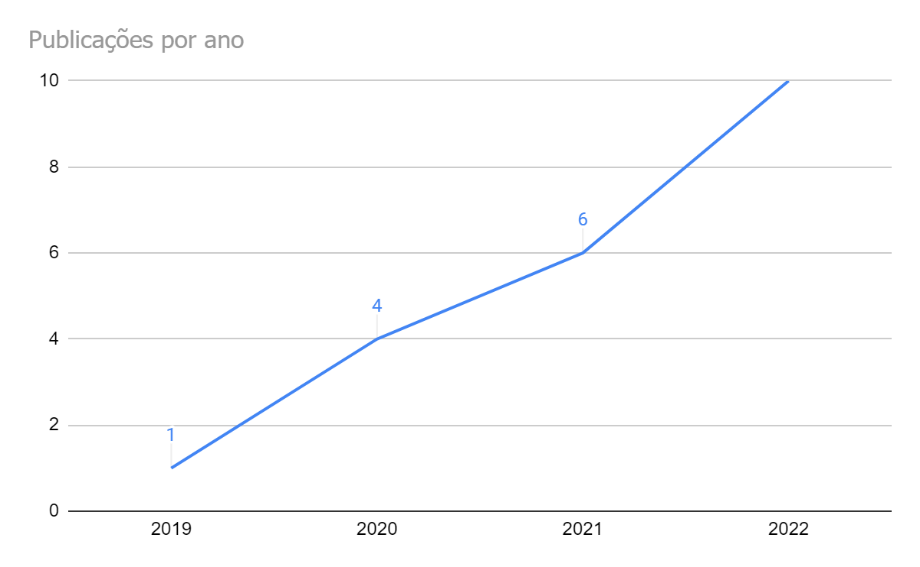
\includegraphics[width=\linewidth]{images/image2.png}
    \caption{Evolución del número de artículos sobre CDD a nivel internacional y número de revistas donde se publican (2010-2023).}
    \label{fig-2}
    \source{Elaboración propia.}
    \end{minipage}
\end{figure}

También se evidencia la extraordinaria hegemonía en este campo de la autoría española, única o compartida (\Cref{tab-3}). En el periodo 2010-2023, el 51,21 \% de los artículos son de autoría exclusivamente española (297 artículos), mientras que la cifra asciende a un 60 \% si tenemos en cuenta también la coautoría con otras nacionalidades (348 artículos). A modo de contexto, el resto de países con más artículos sobre CDD son Noruega (33), Suecia (22), Chile (19), México (21), Alemania (17) o Portugal (15). 

%--- CÓDIGO TABELA 3 ---%
\begin{table}[h!]
\centering
\begin{threeparttable}
\caption{Evolución del número de artículos sobre CDD y artículos con autoría exclusiva y compartida española (2010-2023).} \label{tab-3}
\begin{tabular}{lccc}
\toprule
Periodo & N.º artículos CDD & N.º artículos España & \% Autoría España \\
\midrule
2010 & 23 & 21 & 91,30 \\
2011 & 5 & 4 & 80,00 \\
2012 & 17 & 13 & 76,47 \\
2013 & 11 & 7 & 63,64 \\
2014 & 11 & 7 & 63,64 \\
2015 & 23 & 16 & 69,57 \\
2016 & 19 & 15 & 78,95 \\
2017 & 14 & 10 & 71,43 \\
2018 & 17 & 9 & 52,94 \\
2019 & 29 & 21 & 72,41 \\
2020 & 39 & 29 & 74,36 \\
2021 & 80 & 50 & 62,50 \\
2022 & 159 & 82 & 51,57 \\
2023 & 133 & 64 & 48,12 \\
\addlinespace
Total & 580 & 348 & 60,00 \\
\bottomrule
\end{tabular}
\source{Elaboración propia.}
\end{threeparttable}
\end{table}

Si tomamos como referencia el último periodo analizado (2020-2023), claramente marcado por el COVID-19 y por un interés lógico en asuntos vinculados con la educación digital y la CDD, la producción española sobre CDD representa, con 225 artículos, un 54,74\% de la producción mundial de máximo impacto en esta temática. De hecho, la producción española en CDD se ha triplicado desde el 2019 hasta el 2023, pasando de 21 a 64 artículos y alcanzando los 82 artículos en el 2022 (\Cref{fig-3}).

\begin{figure}[h!]
    \centering
    \begin{minipage}{.8\textwidth} 
    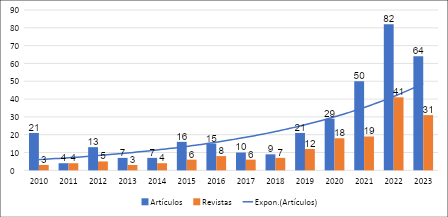
\includegraphics[width=\linewidth]{images/image3.png}
    \caption{Evolución artículos CDD y revistas (autoría y coautoría española).}
    \label{fig-3}
    \source{Elaboración propia.}
    \end{minipage}
\end{figure}

Se constata una alta concentración de la temática en algunas revistas. De hecho, más de la mitad de los artículos (52,41 \%) han sido publicados únicamente en 10 revistas académicas; cinco de las cuales son españolas. No obstante, como podemos observar en la \Cref{tab-4}, el predominio de autoría española no se da únicamente en el caso de revistas españolas como Pixel-Bit o Comunicar; también lo vemos en editoriales de otros países como Sustainability (67,57 \%) o Education Sciences (71,43 \%).

%--- CÓDIGO TABELA 4 ---%
\begin{table}[h!]
\centering
\caption{Ranking de revistas con más artículos (Scopus Q1-Q2 y WoS) sobre CDD ($\geq$ 10) con autoría y coautoría española (2010-2023).}\label{tab-4}
\begin{tabular}{llllll}
\toprule
  & Revista & \multicolumn{1}{>{\raggedright\arraybackslash}p{1.4cm}}{Autoría España (\%)} & \multicolumn{1}{>{\raggedright\arraybackslash}p{1.4cm}}{Autoría coautoría (\%)} & \multicolumn{1}{>{\raggedright\arraybackslash}p{1.4cm}}{País edición} & \multicolumn{1}{>{\raggedright\arraybackslash}p{1.4cm}}{N.º artículos} \\
\midrule
1 & Pixel-Bit & 66,07 & 73,21 & España & 56 \\
2 & Comunicar & 53,33 & 80,00 & España & 45 \\
3 & Education and Information Technologies & 30,23 & 32,56 & EEUU & 43 \\
4 & Education Sciences & 64,29 & 71,43 & Suiza & 42 \\
5 & Sustainability & 64,86 & 70,27 & Suiza & 37 \\
6 & Revista de Educación & 100,00 & 100,00 & España & 19 \\
7 & Nordic Journal of Digital Literacy & 10,53 & 10,53 & Noruega & 19 \\
8 & Educación XX1 & 86,67 & 93,33 & España & 15 \\
9 & Frontiers in Education & 20,00 & 20,00 & Suiza & 15 \\
10 & \multicolumn{1}{>{\raggedright\arraybackslash}p{6cm}}{Journal of New Approaches in Educational Research} & 69,23 & 76,92 & España & 13 \\
\bottomrule
\end{tabular}
\source{Elaboración propia.}
\end{table}



Otro aspecto destacable a partir del análisis de datos sobre CDD, se da en relación con el tipo de metodología utilizada (\Cref{fig-4}), mayoritariamente de tipo cuantitativo. En los últimos cuatro años analizados, el uso exclusivo de metodologías cuantitativas es el predominante, llegando a picos del 94,87 \% y del 91,25 \% durante el año de pandemia y postpandemia (2020-2021). Aunque se podría suponer que, en una situación de confinamiento, con restricciones de movilidad y de distanciamiento físico, el trabajo de campo más lógico en esas circunstancias es el de tipo cuantitativo, hay que decir que en prepandemia se habían llegado a porcentajes similares en 2017 (92,86 \%) o en 2019 (86,21 \%).

\begin{figure}[h]
    \centering
    \begin{minipage}{.8\textwidth} 
    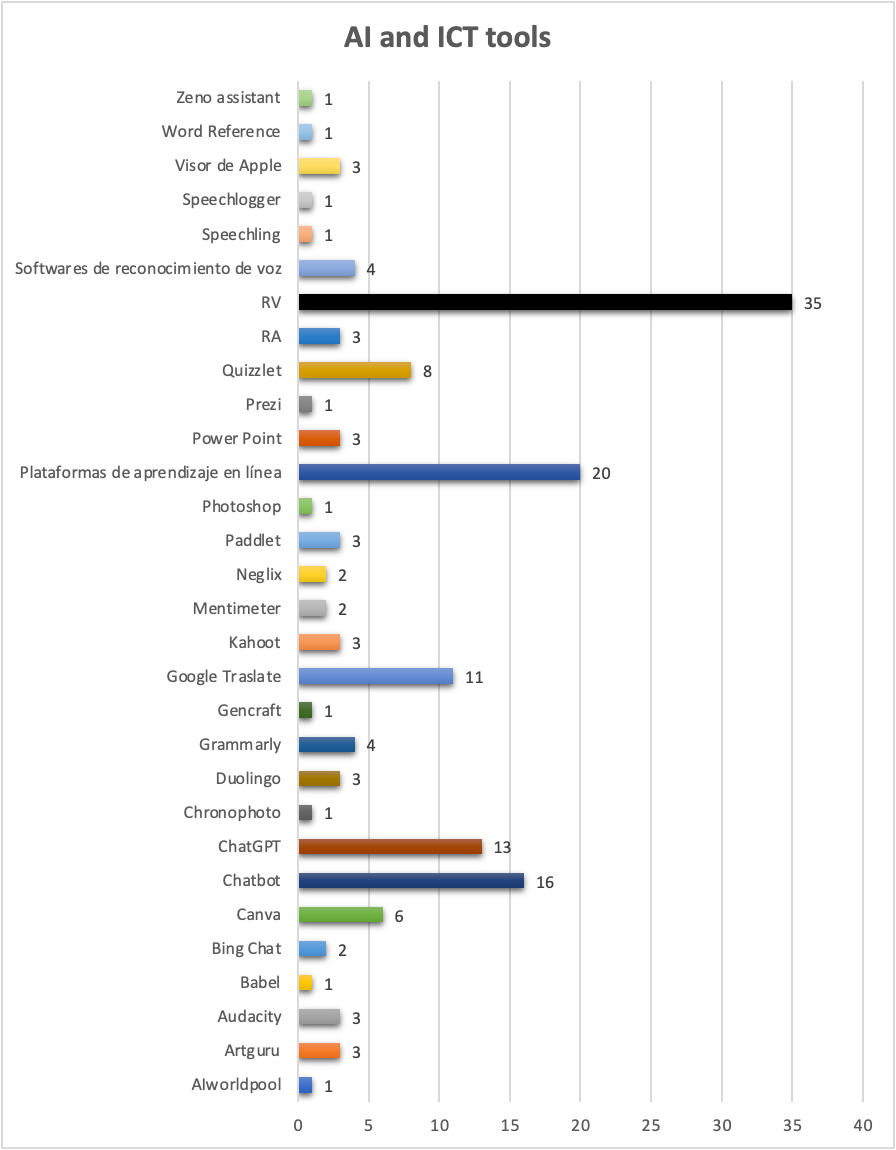
\includegraphics[width=\linewidth]{images/image4.png}
    \caption{Artículos sobre CDD y metodología utilizada (2010-2023).}
    \label{fig-4}
    \source{Elaboración propia.}
    \end{minipage}
\end{figure}

En relación con el tipo de metodología utilizada en materia de CDD, hay que destacar como resultado muy significativo, un cambio de tendencia en los últimos dos años del periodo analizado. Así, y a pesar del monopolio que representa la investigación cuantitativa en este ámbito de estudio, el periodo postpandemia (2022-2023) se caracteriza, a nivel internacional, por un cierto giro hacia investigaciones exclusivamente cualitativas; prácticamente inexistentes, hasta entonces, si tomamos como referencia el periodo analizado (2010-2023). Pese a ello, resulta igualmente significativo que esta tendencia no se observe en la producción científica española sobre CDD; que continúa centrándose casi exclusivamente en estudios de tipo cuantitativo. Como se observa en la \Cref{fig-5}, entre 2022 y 2023 los artículos de autoría española representan un 50 \% de la producción científica internacional en materia de CDD, con 146 artículos. No obstante, mientras que en el resto de países, un 26,71 \% de los artículos publicados en el periodo 2022-2023 han utilizado metodologías cualitativas; en el caso de la publicación de autoría española, el porcentaje se reduce a un 13,01 \%. De este modo, en el periodo postpandemia, un 69,18 \% de la producción científica española en materia de CDD se fundamenta en estudios exclusivamente cuantitativos; mientras que, en el resto de países, decrece el interés por las técnicas cuantitativas para abordar el estudio de la CDD, representando ya solo un 45,89 \%.

\begin{figure}[h!]
    \centering
    \begin{minipage}{.8\textwidth}
    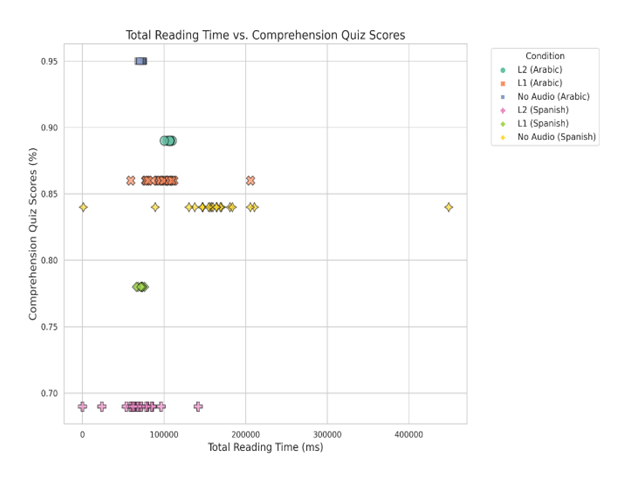
\includegraphics[width=\linewidth]{images/image5.png}
    \caption{Comparativa de la metodología utilizada en la investigación sobre CDD (2022-2023).}
    \label{fig-5}
    \source{Elaboración propia.}
    \end{minipage}
\end{figure}

Dentro de las técnicas cuantitativas, la encuesta es la técnica por excelencia para la investigación en CDD y está presente en un 68 \% de publicaciones internacionales analizadas en el periodo 2010-2023 (\Cref{fig-6}). Si nos fijamos en la producción con autoría española en este mismo periodo, el porcentaje asciende a un 73 \%, mientras que en el resto de países se sitúa en un 60 \% (ver \Cref{fig-7,fig-8}).

\begin{figure}[H]
    \centering
    \begin{minipage}{.5\textwidth}
    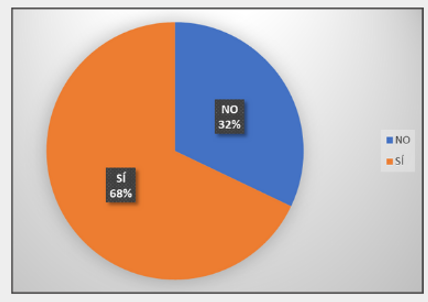
\includegraphics[width=\linewidth]{images/IMAGE6.png}
    \caption{Artículos con encuesta (2010-2023): Producción científica internacional.}
    \label{fig-6}
    \source{Elaboración propia.}
    \end{minipage}
\end{figure}

\noindent
\begin{minipage}[b]{0.42\textwidth}
    \begin{figure}[H]
        \centering
        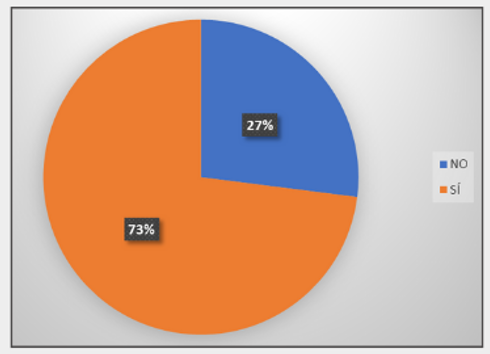
\includegraphics[width=\linewidth]{images/IMAGE7.png}
        \caption{Artículos con encuesta (2010-2023): España.}
        \label{fig-7}
        \source{Elaboración propia.}
    \end{figure}
\end{minipage}
\hfill
\begin{minipage}[b]{0.48\textwidth}
    \begin{figure}[H]
        \centering
        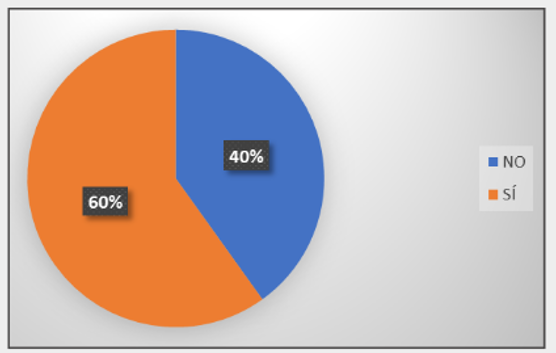
\includegraphics[width=\linewidth]{images/IMAGE8.png}
        \caption{Artículos con encuesta (2010-2023): Resto de países.}
        \label{fig-8}
        \source{Elaboración propia.}
    \end{figure}
\end{minipage}
\bigskip

La producción de artículos sobre CDD exclusivamente con encuestas ha experimentado un crecimiento significativo en estos últimos años (\Cref{fig-9,fig-10}). Solo en el periodo 2017-2023 se producen a nivel global 331 artículos sobre CDD con encuesta. En España, 8 de cada 10 artículos sobre CDD se realizan exclusivamente con encuestas (204 artículos) mientras que en el resto de países son 6 de cada 10 (127 artículos). 

\noindent
\begin{minipage}[b]{0.46\textwidth}
    \begin{figure}[H]
        \centering
        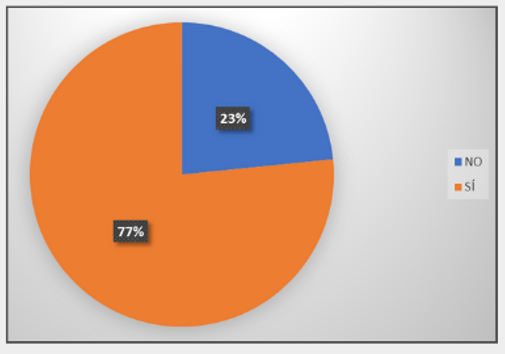
\includegraphics[width=\linewidth]{images/IMAGE9.png}
        \caption{Artículos con encuesta (2017-2023): España.}
        \label{fig-9}
        \source{Elaboración propia.}
    \end{figure}
\end{minipage}
\hfill
\begin{minipage}[b]{0.50\textwidth}
    \begin{figure}[H]
        \centering
        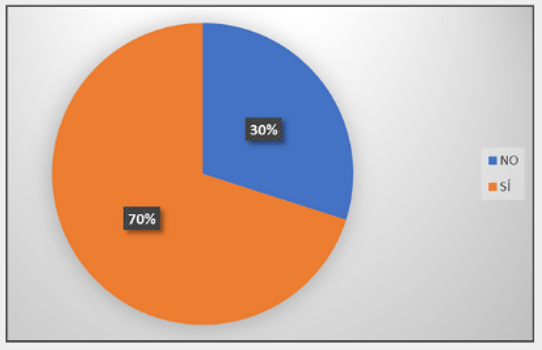
\includegraphics[width=\linewidth]{images/IMAGE10.png}
        \caption{Artículos con encuesta (2017-2023): Resto de países.}
        \label{fig-10}
        \source{Elaboración propia.}
    \end{figure}
\end{minipage}
\bigskip

Se podría pensar que en este último periodo el uso de encuestas se produce, en gran medida, durante el periodo de pandemia y postpandemia, debido al consabido confinamiento, el auge de la educación virtual, remota y online, las llamadas a mantener una cierta distancia social o las dificultades y restricciones en la movilidad. Pues bien, aunque esto es así para el caso de España no es, ni mucho menos, la tendencia a nivel internacional (ver \Cref{fig-11,fig-12}). Mientras que durante dicho periodo el volumen de artículos con autoría o coautoría de España es del 82 \%, en el caso del resto de países el porcentaje es solo del 64 \%.

\noindent
\begin{minipage}[b]{0.50\textwidth}
    \begin{figure}[H]
        \centering
        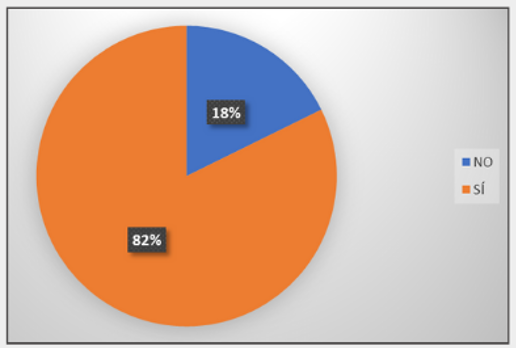
\includegraphics[width=\linewidth]{images/IMAGE11.png}
        \caption{Artículos con encuesta (2017-2023): España.}
        \label{fig-11}
        \source{Elaboración propia.}
    \end{figure}
\end{minipage}
\hfill
\begin{minipage}[b]{0.49\textwidth}
    \begin{figure}[H]
        \centering
        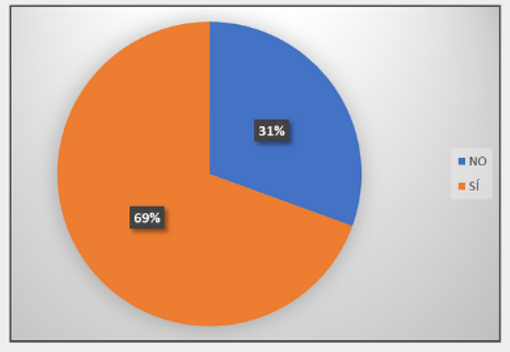
\includegraphics[width=\linewidth]{images/IMAGE12.png}
        \caption{Artículos con encuesta (2017-2023): Resto de países.}
        \label{fig-12}
        \source{Elaboración propia.}
    \end{figure}
\end{minipage}
\bigskip

Con relación a las encuestas, las muestras seleccionadas son muy reducidas (\Cref{fig-13}). Más de la mitad de las publicaciones (53,81 \%) se han llevado a cabo con encuestas realizadas a menos de 400 sujetos. 

\begin{figure}[h!]
    \centering
    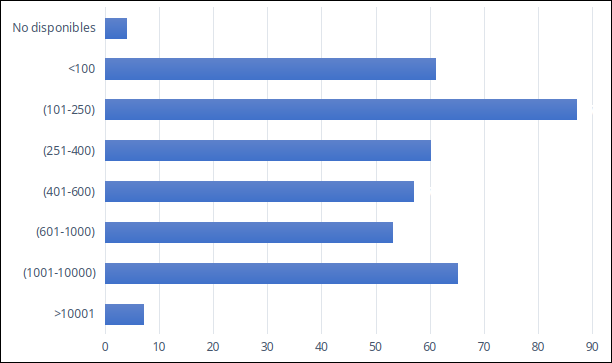
\includegraphics[width=0.75\linewidth]{images/IMAGE13.png}
    \caption{ Artículos CDD con encuesta (2010-2023) según tamaño de la muestra.}
    \label{fig-13}
    \source{Elaboración propia.}
\end{figure}

Si nos centramos en el diseño de encuestas, en nuestro análisis se demuestra que un porcentaje extraordinario se ha llevado a cabo con un carácter intencional, con muestras no probabilísticas y excesivamente fragmentadas y reducidas. A modo de ejemplo, hemos seleccionado todos los artículos que incorporan encuestas con $\geq 205 \leq 240$ sujetos (\Cref{tab-5}). Observamos que, no solo las muestras son demasiado reducidas -- y, por tanto, hay que ser muy prudente con los resultados y no derivar de ellos grandes conclusiones \textendash, sino que, además, las muestras que se han utilizado son muy dispersas: estudiantes universitarios de Grado o de Máster en Educación de una sola universidad, profesorado universitario de una o de varias universidades (españolas o sudamericanas), maestros de educación infantil, primaria, secundaria o profesorado universitario de diferentes regiones o estados. En el conjunto del periodo, la mayor parte de las muestras se ha seleccionado entre el profesorado y el alumnado universitario de educación (futuro profesorado). Este hecho resulta paradójico si se tiene en cuenta que el marco normativo y legislativo español se ha centrado en la acreditación y certificación de las competencias del profesorado no universitario. 

%--- CÓDIGO TABELA 5 ---%
\begin{small}
\begin{longtable}{>{\raggedright\arraybackslash}p{2.5cm} l >{\raggedright\arraybackslash}p{6cm} ll}
\caption{Artículos CDD con población y muestras $\geq 205 \leq 240$ sujetos.}\label{tab-5} \\
\toprule
Revista & Año & Población y muestras & Autoría & Muestra \\
\midrule
Comunicar & 2010 & Estudiantes de Magisterio (Universidad de La Rioja, España) & España & 205 \\
Sustainability & 2022 & Estudiantes Máster Secundaria (Universidad Politécnica de Madrid, España) & España & 207 \\
Revista de Educación & 2012 & Estudiantes Formación inicial del profesorado (Universidad de León, España) & España & 212 \\
Pixel-Bit & 2022 & Profesorado Universidad (Universidad Pablo de Olavide, España) & España & 214 \\
Education Sciences & 2021 & Profesorado Universidad (Ecuador) & España/Ecuador & 216 \\
Electronics & 2021 & Profesorado Universidad (Sudamérica) & España & 219 \\
Revista de Educación a Distancia & 2023 & Profesorado de Universidad (España) & España & 220 \\
Sustainability & 2021 & Estudiantes Máster Secundaria (Universidad de Jaén, España) & España & 220 \\
European Journal of Education & 2022 & Profesorado de Secundaria de Indonesia & Indonesia & 221 \\
Pixel-Bit & 2015 & Estudiantes Grado Educación Infantil y Primaria (Universidad de Castilla-La Mancha, España) & España & 224 \\
Comunicar & 2015 & Profesorado Infantil y Primaria Alicante (España) & España/EEUU & 224 \\
Comunicar & 2022 & Estudiantes Grado (Universidad de Burgos, España) & España & 225 \\
International Journal of Evaluation and Research in Education & 2022 & Estudiantes y profesorado de Indonesia & Indonesia & 233 \\
Frontiers in Education & 2022 & Estudiantes Grado Educación Primaria (Universidad de Navarra, España) & España & 235 \\
Journal of New Approaches in Educational Research & 2023 & Profesorado de Posgrados Universitarios (Universidad de La Laguna, España) & España & 239 \\
Revista Interuniversitaria de Formación del Profesorado & 2022 & Profesorado Universidad (Chile) & España/Chile & 239 \\
Pixel-Bit & 2011 & Profesorado Educación Infantil Sur de Sonora & México & 240 \\
\bottomrule
\source{Elaboración propia.}
\end{longtable}
\end{small}

\section{Discusión y conclusiones}\label{sec-4}

La originalidad de la investigación radica en que en ella convergen la voluntad de situar la investigación española en CDD en el contexto internacional, de una parte, y la voluntad de señalar algunos retos de futuro de la investigación en este ámbito. Además, tanto la muestra de artículos que hemos analizado como el periodo tenido en consideración, es uno de los más amplios que se ha realizado en un artículo de estas características. Se trata, en definitiva, de vislumbrar las luces y sombras de un monopolio, atípico, en un determinado ámbito de conocimiento. 

De la investigación realizada se concluye que la CDD ha sido un objeto de estudio con un crecimiento extraordinario, tanto en España como a nivel internacional, durante las últimas dos décadas. Uno de los principales factores que explican dicho crecimiento ha sido el impulso generado a partir de diferentes normativas y marcos de referencia tanto de ámbito estatal como a nivel internacional. En el caso español se ha generado un marco normativo legal partiendo de dichos marcos normativos \cite{boe2022b, boe2022a, intef2017, redecker2017, unesco2018}.

La selección y análisis exhaustivo de 580 artículos en torno a la CDD, junto con los principales marcos de referencia para abordarla, nos ha permitido corroborar, incluso superando las expectativas iniciales, la primera hipótesis sobre el predominio de los y las investigadoras en este ámbito de estudio (H1). La investigación española sobre CDD monopoliza la publicación en dicha materia a nivel mundial desde el inicio del periodo analizado. Este hecho se constata en el liderazgo de la autoría en el conjunto del periodo. Además, en el ranking de revistas académicas que más publican sobre la temática hay cinco que son españolas.

A partir de los datos analizados se corrobora también la H2. Se demuestra el predominio de los análisis cuantitativos sobre los de tipo cualitativo \cite{peters2022}. Así, partiendo del análisis de 580 artículos sobre CDD, no deja de ser sorprendente que siete de cada diez artículos se hayan llevado a cabo mediante encuestas. En este sentido, los resultados son muy desiguales en cuanto a la población y las muestras elegidas \cite{ballano2024, zhao2021}. En este sentido, se constata que dichas encuestas, mayoritariamente, pretenden medir la autopercepción del profesorado o del futuro profesorado, pero a partir de encuestas no probabilísticas, con muestras excesivamente reducidas, con una gran fragmentación de públicos y con datos, por tanto, no generalizables. No es solo que exista un abuso de investigaciones con metodologías exclusivamente basadas en encuestas, sino que la mayoría no nos permiten plantearnos más que conclusiones, en el mejor de los casos, parciales y sesgadas. Asimismo, en el apartado metodológico, hemos señalado que uno de los aspectos más complejos de identificar ha sido la población objeto de estudio. Para analizar la percepción de la CDD del profesorado de enseñanza primaria y secundaria es recurrente tomar como objeto de estudio lo que hemos denominado futuro profesorado: estudiantes de grados y másteres en educación. Esto ocurre sin la certeza de que el conjunto de dichos colectivos acabe ejerciendo como profesorado de primaria y secundaria. Evidentemente, resulta más sencillo para los y las investigadoras acceder al alumnado propio de grado o postgrado de educación (futuro profesorado), en vez de realizar encuestas directamente a docentes de educación infantil, primaria, secundaria o ciclos de formación profesional. Por otro lado, en ciencias sociales, siempre ha existido un cierto complejo de inferioridad y algunas disciplinas académicas han preferido utilizar métodos cuantitativos para así acercarse a una supuesta cientificidad en sus propuestas \cite{busquet2017}.

También la H3 queda corroborada, ya que en el periodo 2020-2022, en un contexto de confinamiento, restricciones a la movilidad y auge de la virtualidad en el sector educativo debido a la pandemia mundial, la publicación sobre CDD ha crecido de manera exponencial. No obstante, durante 2023, pese a que el número de artículos sobre la temática continúa siendo elevadísimo, se trata del primer año, desde 2017, en que se observa un retroceso en la publicación sobre CDD. Aun así, solo en 2022 y 2023 se han publicado 292 artículos, la mitad de los producidos en el conjunto del periodo (2010-2023). En este punto, hay que destacar algunos aspectos novedosos. Por un lado, observamos que el monopolio de la investigación española no es tan claro como en años anteriores. Por otro lado, pese a que la investigación española continúa utilizando casi exclusivamente la encuesta como método prioritario de trabajo de campo, en el resto de países que publican sobre la temática van tomando fuerza los análisis de tipo cualitativo. 

Otra conclusión significativa que se deriva de nuestro análisis es la existencia de un importante sesgo entre, por un lado, la evolución de los marcos de referencia y legislación que han impulsado el establecimiento de los indicadores para el reconocimiento de la CDD en educación primaria y secundaria \cite{boe2022b}; y, por otro lado, una investigación basada casi exclusivamente en la percepción de la CDD partiendo de su conocimiento y uso en entornos de educación superior \cite{ballano2024, fernandezbatanero2021}. Este aspecto es esencial para continuar profundizando en la formación, así como en los niveles de evaluación y acreditación de la CDD del profesorado universitario \cite{barragan2021, barragan2024, caberoalmenaraetal2020, domingocoscollola2020}.

Por otro lado, tanto los estudios que pretenden medir la CDD mediante encuestas, como los marcos de referencia para establecer modelos de evaluación y acreditación de la CDD, han tendido a equiparar tener una determinada CDD con el uso de las tecnologías en las aulas \cite{alvarez2015}. Este hecho resulta, como mínimo, discutible \cite{castaneda2018, ramirez2012}. El binomio conocer/utilizar denota más un modelo que pretende medir la inserción de las TIC en los centros educativos en lugar de medir la CDD del profesorado. No utilizar un determinado programa, redes o tecnología se puede deber a una infraestructura tecnológica escasa y deficiente o simplemente a un criterio didáctico. A su vez, el uso de determinada tecnología en el aula no garantiza, necesariamente, estar en disposición de dicha competencia. Constatamos que en este aspecto radica una de las principales problemáticas y retos de la investigación sobre CDD.

Las limitaciones de este estudio tienen que ver con las propias de cualquier acotación metodológica. En primer lugar, podemos identificar una limitación de tipo temporal que tiene que ver con el periodo analizado (2010-2023). Aun siendo muy amplio y representativo, este periodo excluye las publicaciones anteriores al 2010 y las realizadas a partir de 2024. En segundo lugar, se han excluido los artículos que no estaban en castellano o inglés, con acceso abierto o indexados con criterios diferentes para su inclusión en esta investigación. Finalmente, por limitaciones de espacio, se puede apuntar que, dado el gran volumen de documentos, artículos y variables analizadas, no se han podido tratar o desarrollar en este artículo otros resultados que tienen relación con, por ejemplo, el análisis de la evolución de la producción científica sobre CDD en función de la universidad de origen de los artículos analizados o, por otro lado, un análisis más detallado de la evolución de los marcos de referencia sobre la CDD. 

Pese a ello, consideramos que los resultados y las conclusiones que se desprenden son muy significativos para la comunidad científica. Como líneas de investigación futuras, hay que seguir profundizando en los análisis que permitan discernir las diferencias entre conocimiento y uso para identificar una determinada competencia. Así, resulta clave entender que no utilizar tecnología no implica no tener el conocimiento sobre ella. Pueden ser otros factores los que impidan o dificulten su uso, que, de ninguna manera, implica un no conocimiento o no tener habilidad o destreza, es decir competencia, en este caso digital. En este punto, es imprescindible poder discernir un estado de la cuestión sobre la situación real de la competencia digital del profesorado. Cualquier diseño formativo requiere de un análisis certero de la situación actual. Por tanto, se hace imprescindible realizar investigaciones, tanto cualitativas como cuantitativas, que no establezcan relaciones causales directas entre usar y poseer una determinada competencia. Y ya que actualmente existe en España un marco para la acreditación de la CDD del profesorado no universitario, dichos estudios tendrían que focalizarse tomando como objeto de estudio prioritario dicha población. Por otro lado, hay que examinar la CDD de los docentes universitarios y trabajar en los indicadores que permitan, en un futuro, el desarrollo de marcos normativos para su certificación. Pero, no se trata de trasladar para la enseñanza universitaria el modelo de certificación de la CDD ya aprobado \cite{boe2022b}. Este establece niveles competenciales graduales y está basado fundamentalmente en la tenencia de certificados, la obtención de títulos, el desarrollo de cargos unipersonales o la aportación de evidencias como premios, publicaciones científicas o la elaboración de proyectos \cite{generalitat2023}. Al contrario, se podría establecer un modelo de certificación más competencial, más integral, basado en la experiencia profesional, con la participación de responsables y alumnado y directamente relacionado con la detección de necesidades formativas reales e inmediatas del profesorado y totalmente conectado con procesos de innovación pedagógica. Al contrario, se podría establecer un modelo de certificación más competencial, más integral, basado en la experiencia profesional, con la participación de responsables y alumnado y directamente relacionado con la detección de necesidades formativas reales e inmediatas del profesorado y totalmente conectado con procesos de innovación pedagógica.

Resulta vital, como hemos demostrado en este artículo, que cuando se realicen investigaciones cuantitativas sobre el conjunto del profesorado se hagan con rigor y utilizando muestras probabilísticas y representativas. Siendo complejo, en ocasiones, disponer para la investigación de dichas muestras, hay que seguir trabajando en aportaciones de tipo cualitativo que podrán aportar matices y riqueza en el análisis de la percepción de la CDD. Asimismo, el desarrollo de la IA está transformando completamente todos los ámbitos, incluido el educativo. Su impacto en los procesos de enseñanza-aprendizaje o, de manera específica, en las metodologías y en los procesos de evaluación, hace necesaria una actualización de los procesos de certificación de la CDD. La mayoría de los elementos que hemos estudiado vinculados a la competencia digital, no únicamente del profesorado, se verán totalmente modificados por la irrupción y desarrollo de la IA. 


\printbibliography\label{sec-bib}
% if the text is not in Portuguese, it might be necessary to use the code below instead to print the correct ABNT abbreviations [s.n.], [s.l.]
%\begin{portuguese}
%\printbibliography[title={Bibliography}]
%\end{portuguese}


%full list: conceptualization,datacuration,formalanalysis,funding,investigation,methodology,projadm,resources,software,supervision,validation,visualization,writing,review
\begin{contributors}[sec-contributors]
\authorcontribution{Alfons Medina Cambrón}[formalanalysis,conceptualization,writing,review,investigation,methodology,resources,supervision,validation]
\authorcontribution{Sonia Ballano Macías}[formalanalysis,conceptualization,writing,review,investigation,methodology,resources,supervision,validation]
\end{contributors}



\end{document}

